\section{Analysis}
This section contains the analysis of app functionality, Android app development, \gls{rs} algorithms and communication with the aSTEP system.

%temporary title
\subsection{App functionality}
% meta shit
The app user interface is a low priority task during this project.
However, the app needs basic functionality, according to the requirements.

% User management
To be able to separate different routes, and to assign them to their respective users, there has to be a user management system, so that each user has its own ID.

% Ride matches
The user should also be informed with relevant information of ride matches, so that the user can make a decision of sharing a ride or not.

% User settings
The user of the application should also be able to adjust their settings.
The settings are preferences regarding different properties of ride sharing.
The user should be able to decide if it wants to get a ride or give a ride or both.
There are also properties of the user itself, like a description and a picture, that other users can access to decide if they want to share a ride with the named user.



% other shit...



\subsection{Android Development Platform}
When developing Android applications one of the first choices to consider is which API levels to target \cite{usesSDK}.
The ``\textit{API Level is an integer value that uniquely identifies the framework API revision offered by a version of the Android platform.}'' according to Android Developers \cite{usesSDK}.
The distribution of the Android version levels are shown in \ref{fig:dashboard}.

``\textit{The manifest file presents essential information about your app to the Android system, information the system must have before it can run any of the app's code.}'', according to Android Developers \cite{androidManifest}.
The manifest requires to specify the API level for three definitions: minimum, target and maximum. 
The target and max versions requires few consideration to determine.
The ``targetSdkVersion'' reflects the version to which the app is developed and tested against, without enabling compatibility behaviors.
The ``maxSdkVersion'' reflects the highest API level that an app is designed to run.
Both of these are set to the highest API level available during the start of the development, which is API version 23.

\begin{figure}[h!]
	\centering
	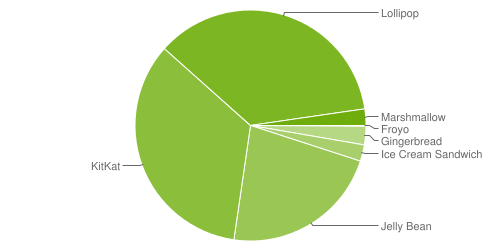
\includegraphics[width=0.7\textwidth]{figures/android-chart-march.png}
	\caption{Android version distribution, March 2016 \cite{androidDashboard}}
	\label{fig:dashboard}
\end{figure}

The last API level which needs to be specified is the ``minSdkVersion''.
This entry specifies the lowest API level which an app supports.
A cause of this is that every device with an API level lower than the specified minSdkVersion will not be compatible with the app.
Supporting older API versions requires development efforts, typically implementing functionality though the Android Support Library \cite{androidSL}.
For this project we choose to target a higher API level for to simplify the development process.
At the time of writing, the platform version distribution sum of API levels greater than or equal to 21 (Android Lollipop) is 35,3\%.
API version 21 is chosen as the minSdkVerison, the main reason for this choice is to minimize development time for user interface, as API level 21 added support for Android's new material design style \cite{android5API}. Refraining from further backwards compatibility allows the project focus to be on the functionality of the app. 

\subsection{Periodic Background Tasks}\label{ssec:periodictasks}
When the app is installed on the device, the app needs to run a task to periodically collect location data.
\Citet{friesen2015android} writes how this can be done in the Android API by utilizing the AlarmManager and the JobSchedular.

\paragraph{AlarmManager}
The AlarmManager was created to handle alarms, and implemented as a general class that can call any task after one or multiple given time periods.
The alarm can be set to be reoccurring, thus gather a location with the given interval.

\paragraph{JobScheduler}
The JobScheduler was implemented in Android 5.0 (API 21) as an alternative to the AlarmManager.
The scheduler behaves in a similar way as the AlarmManager, but tries to batch the jobs together and execute them in bundles.
This means that the device can save power by avoiding going to sleep just to wake a short moment later, on the cost of time precision. 
While the AlarmManager has the option to occur at a exact time, the JobSchedular does not.

The JobScheduler is chosen as the basis for the background tasks, because the timing accuracy of the location data is not sensitive to minor deviations, in addition to the advantages of saving power features.

\subsection{Location tracking}\label{ssec:loctrack}
% metatext
In order to be able to locate a user and to construct routes, it is necessary to collect location data. 
Such collection of locations can be done by using already existing services, such as the Google Play Services.

% something
Location data in \gls{rs} is formatted in decimal coordinates in an array that represents a route from A to B.
There are several ways to collect location data. 
One of them is to manually develop a component to do so on the Android device, but the chosen solution is to utilize the already existing Google Play Services.

To use Google Play Services, a client library must be included in the app, and will communicate via inter-process communication to the Google Play Services. 

An advantage of the Google Play Services \cite{GapiOverview}, is that it will automatically receive silent updates regularly, to acquire new features and bug fixes to the used services, developed by Google, and this is illustrated in Figure \ref{fig:gapifigure}.
The Google Play Services are restricted, and are not supporting devices with Android versions lower than 2.3. 
This limits the backwards compatibility, but the app is already restricted to Android 5 and newer, and has no influence on the target audience.

\begin{figure}[h]
	\centering
	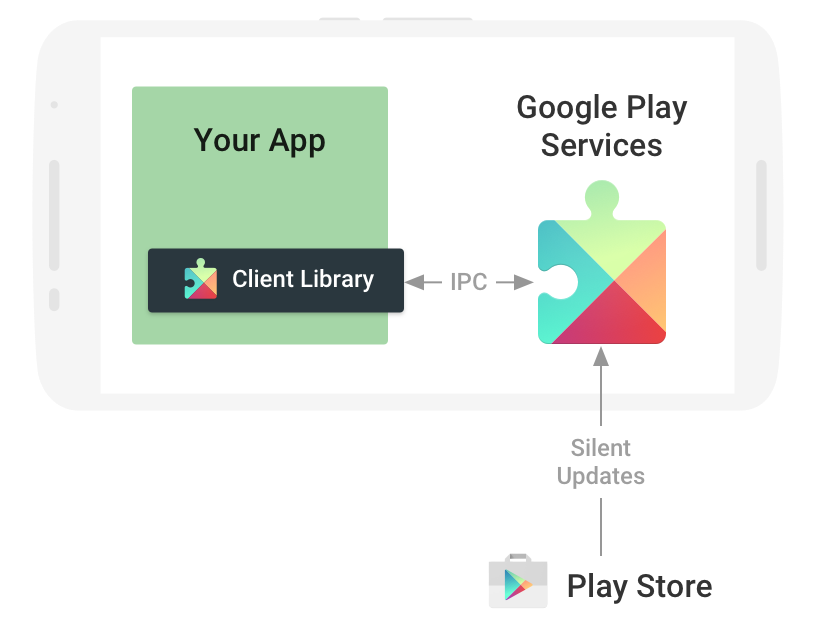
\includegraphics[width=0.7\textwidth]{figures/play-services-diagram.png}
	\caption{Google Play Services communication\cite{GapiFigure}}
	\label{fig:gapifigure}
\end{figure}

The Google Play Services will allow the application to collect location data, but it is not doing so solely by using the GPS in the device. 
The location service utilizes both network location and GPS to estimate a position as precise as possible \cite{GapiLocation}. 
To ensure the collected location data is relevant, locations are only collected when the user is traveling by vehicle.

The Google Play Services provides a service to determine the user's activity, called Activity recognition. 
Activity recognition is a service that utilizes several sensors on the device to determine what kind of activity the user is currently performing, therein driving, walking, etc.
The service will return a probability level from 1 to 100, where 100 is certain that a user is performing the activity.
The activity recognition will also prevent unnecessary data will be stored on the database. 

The practical design of the location tracking and activity recognition will be further explored in the following design section.
The \gls{astep} system is examined as an external tool, and its functionalities are explored.

% algorithm analysis if necessary
\subsection{Algorithms for ridesharing}


% aSTEP system functionality analysis: communication with aSTEP
\subsection{Communication with \gls{astep}}\label{ssec:communicationwithastep}
To be able to utilize the \gls{astep} system, the communication protocol and its functions must be analyzed. 
The analysis is based on the current development and plan of the API and other functions.

% \gls{astep} organization - groups
The intended functions are established in collaboration with other project groups responsible for the \gls{astep} system side of the development. 
%We are mainly involved with the user management group and outdoor location based services groups.

% What does the \gls{astep} system look like?
The design of the \gls{astep} system is currently consisting of an API that apps and services can communicate with, and a backend with user management and location based services, which is stored in a database system.
However, the only relevant part for the \gls{rs} solution is the API, as the internal parts of the \gls{astep} core are administrated by other groups, and are not available through the API.

% What is stored in \gls{astep}
The \gls{astep} system will store information regarding location data, and basic user information. 
The data stored in the \gls{astep} system, relevant to this project solution, is:
\begin{itemize}
	\item Location data consisting of userID, routeID, GPS coordinates and timestamp.
	\item Username
	\item Password
\end{itemize}

The \gls{astep} user management system does not provide storage of data regarding contact information for \gls{astep} users.
The only information stored is a username and password to keep the \gls{astep} core as simple as possible.
Additional information that is required to make the app work as intended is each of the app groups own responsibility.
The \gls{astep} users are made to ensure the correct permissions are given to the correct user and so that the appropriate data is returned to each user.
An API call cannot be done without the user first being authenticated with a valid login.

% How to cummunicate with \gls{astep}
The communication with \gls{astep} is done through a REST API over HyperText Transfer Protocol, decided in agreement between the \gls{astep} project groups.
REST is an abbreviation of Representational State Transfer, and is a communication design often used in for HTTP-communication \cite{REST}.
Accordingly, the communication is performed by making queries to the \gls{astep} system. 
All communication must be done as a request from the device, to which the \gls{astep} server will respond.

% api functions
The currently available API functions at this stage of the development of \gls{astep} from user management and location services can be seen in Table \ref{tab:sprint2-api}.
The API is providing a POST-request under the name ``PostLocationDat'', as listed in \ref{tab:sprint2-api}, which is the current method to use when sending location data to the \gls{astep} system.
The call will accept location data as a coordinate consisting of longitude and latitude, a precision value, and a value representing time of day in milliseconds.

\begin{table}[!ht]
	\centering
	\begin{tabular}{ll}
		LBS & UM    \\
		\hline
		\begin{tabular}[t]{@{}l@{}}
			GetAllEntitiesInArea\\ GetAllEntitiesInTimePeriod\\ GetAllGroupMemebersLocationAndName\\ GetAllFriendsInArea\\ GetAllFriendsInRadius\\ GetAllGroupMembersInArea\\ GetAllGroupMembersInRadius\\ PostLocationData\end{tabular}
		&
		\begin{tabular}[t]{@{}l@{}}
			Create user\\ Get token\\ Update password\\ Edit privacy settings\\ Allow user2 to access user1's info\end{tabular}
	\end{tabular}
	\caption{Currently planned \gls{astep} API functions.}
	\label{tab:sprint2-api}
\end{table}


As both the \gls{astep} service and Android system have been analyzed it is possible to establish a set of requirements for the second sprint.

% Sprint 2 krav
\subsection{Requirements for the second sprint}
%meta
Sprint two is the first of the two middle sprints that have implementation as the primary focus. In this section, the main issues to be solved in the current iteration will be presented.

% algorithm
\textbf{Route Matching Algorithm}\\
In this sprint, the algorithm for comparing routes must be researched and developed. 
It should be developed to an extent so that it is constructed as pseudocode of the algorithm, to be handed over to another \gls{astep} group, and be implemented in the \gls{astep} system.

\textbf{User Data}\\
User information such as username, password, and login token, must be analyzed to figure out where this information should be stored, and how it should be handled regarding communication between the application and the aSTEP server. 

\textbf{RideShare app}\\
A base for the functionalities for the \gls{rs} application should be implemented. 
The implementation should include a working \todo{?} including of the Google Play Services and the application should be able to collect and store location data. 
The application should also have functionality to run as a background services, so that location data can be collected at all times.

\textbf{System Architecture and Communication}\\
Communication between the \gls{rs} application and \gls{astep} server should also be researched and an implementation of the communication should be initialized in this iteration, ensuring the next iteration will have a base for communication. 
It should be considered how to handle storing the collected location data and how much should be stored where, either on the device or on the \gls{astep} server.

\textbf{Mock Data}\\
If there is spare time during the sprint, it should be considered to acquire mock up location data related to mock up users. 
This data could be used in the third iteration to test if the algorithm works as intended.